\chapter{Introduction}
\label{chap:01_introduction}

% \todo[inline]{
% Margins needs to be reduced back in layout.tex to
% "oddsidemargin 2.7cm", "evensidemargin 2.6cm"
% and "usepackage[paperwidth=275.9mm, paperheight=279.4mm]{geometry}"
% in Thesis.tex needs to be removed.}

% - why other theories do not fit into this problem (like finger printing, beam forming)
% -> TDOA between robots -> one does not want to send signal samples
%    via message. (Too large information)
%   -> Approach of Dortmund -> too inaccurate time point when whistle is detected. NTP too
%      inaccurate, offline synchronization can be done or PTP implementation
% Another approach would be the TDOA between the robots. Therefore, the robots needs to
% be synchronized in time. The whistle detection time point can then be taken for calculating
% the time difference of arrival. The distance between the robots needs to be known
% Robots needs to be synchronized (which is difficult with NTP only)

\unsure[]{
\acf{SSL} of audio signals is a present subject of research due to increasing
has been subject of research for many years with application
scenarios in various environments and applicability to a wide range of
different sensors}
\todo{Chen2006, cite, cite}
\todo{Maybe enumerate two examples explicitly with "environment",
"sensor used" and citation. E.g. Application domains range from X where SSl is
applied on Y-sensor-data to achive Z, to ....}
% In particular for audio signals, use cases emerge with the progressing
% ordinariness of technical equipment on a daily basis.\todo{What do you mean by
% this sentence?}
% As technical devices gained in importance more and more,
Assuming robots as forthcoming everyday objects, reaction to acoustic
input is one essential step for natural human-robot interaction \cite{audio_loca_robotics,socially_interactive_robots}.
Additionally from robots' perspective, various information about the environment
helps to manage unknown scenarios.
For example, navigating robots being aware of obstacles beforehand
due to acoustic perception is a beneficial ability \cite{robust_localization_sources}.
An even more tangible case can be seen in conference rooms of business environments
where remote participation is commonplace these days.
Special features of communication systems like speaker identification and tracking
become crucially important to provide smooth operation \cite{Brandstein96apractical}.
In general, \ac{SSL} algorithms can be divided into three categories
which are based on beamforming, eigenvalue
decomposition or \ac{TDOA} \cite{Brandstein96apractical,gcc_time_broeck,benesty_passive_acoustic}.

In this work, the performance of different \ac{SSL} strategies is evaluated
with a focus on whistle sound localization in the context of the
\textit{\acs{RoboCup} \ac{SPL}}.
As stated in \cite{BAS_estimator}, beamforming methods are computationally
expensive and eigenvalue decomposition is little suitable for signals with
small bandwidth. For an application in the \acs{RoboCup} domain, these constraints
are undesirable as this setting requires real time processing of low-bandwidth
whistle signals.
Therefore, in this work the \ac{TDOA} method was selected as the
most appropriate solution.

A widespread approach to compute the \ac{TDOA} is to cross-correlate the sensor
readings of two microphones to recover the time delay between both channels\cite{brandstein_robust_method}.
By this, the relative direction of a signal source can be obtained from
geometric reasoning on a single robot. From multiple such direction estimates
a global sound source position can be estimated.

\section{Motivation}

The \acf{RoboCup} promotes research on autonomous robotic systems
by hosting competitive events for  scientists and students from around the
world.
It provides a platform that focuses on fast intelligent systems and multi-agent
collaboration \cite{robocup}. This initiative encourages young engineers to
work in real case scenarios by providing several leagues focusing on different
engineering challenges relevant to the field of robotics.

In the \ac{RoboCup} \acf{SPL}, software for humanoid robots is developed to
play soccer autonomously for scientific purpose.
According to the rules of this league, all competitors are constraint to use the
same hardware platform and no modifications are allowed. By this means, the \ac{SPL}
provides a competitive algorithmic real world benchmark.
Since 2008 commercially available humanoid \textit{NAO} robots by the company
\textit{SoftBank Robotics} are the official standard platform in this league.
They are equipped with a variety of different sensor like cameras, speakers,
microphones, sonars and many more.
% -------------------------------------------------------------
\begin{figure}[ht]
	\centering
        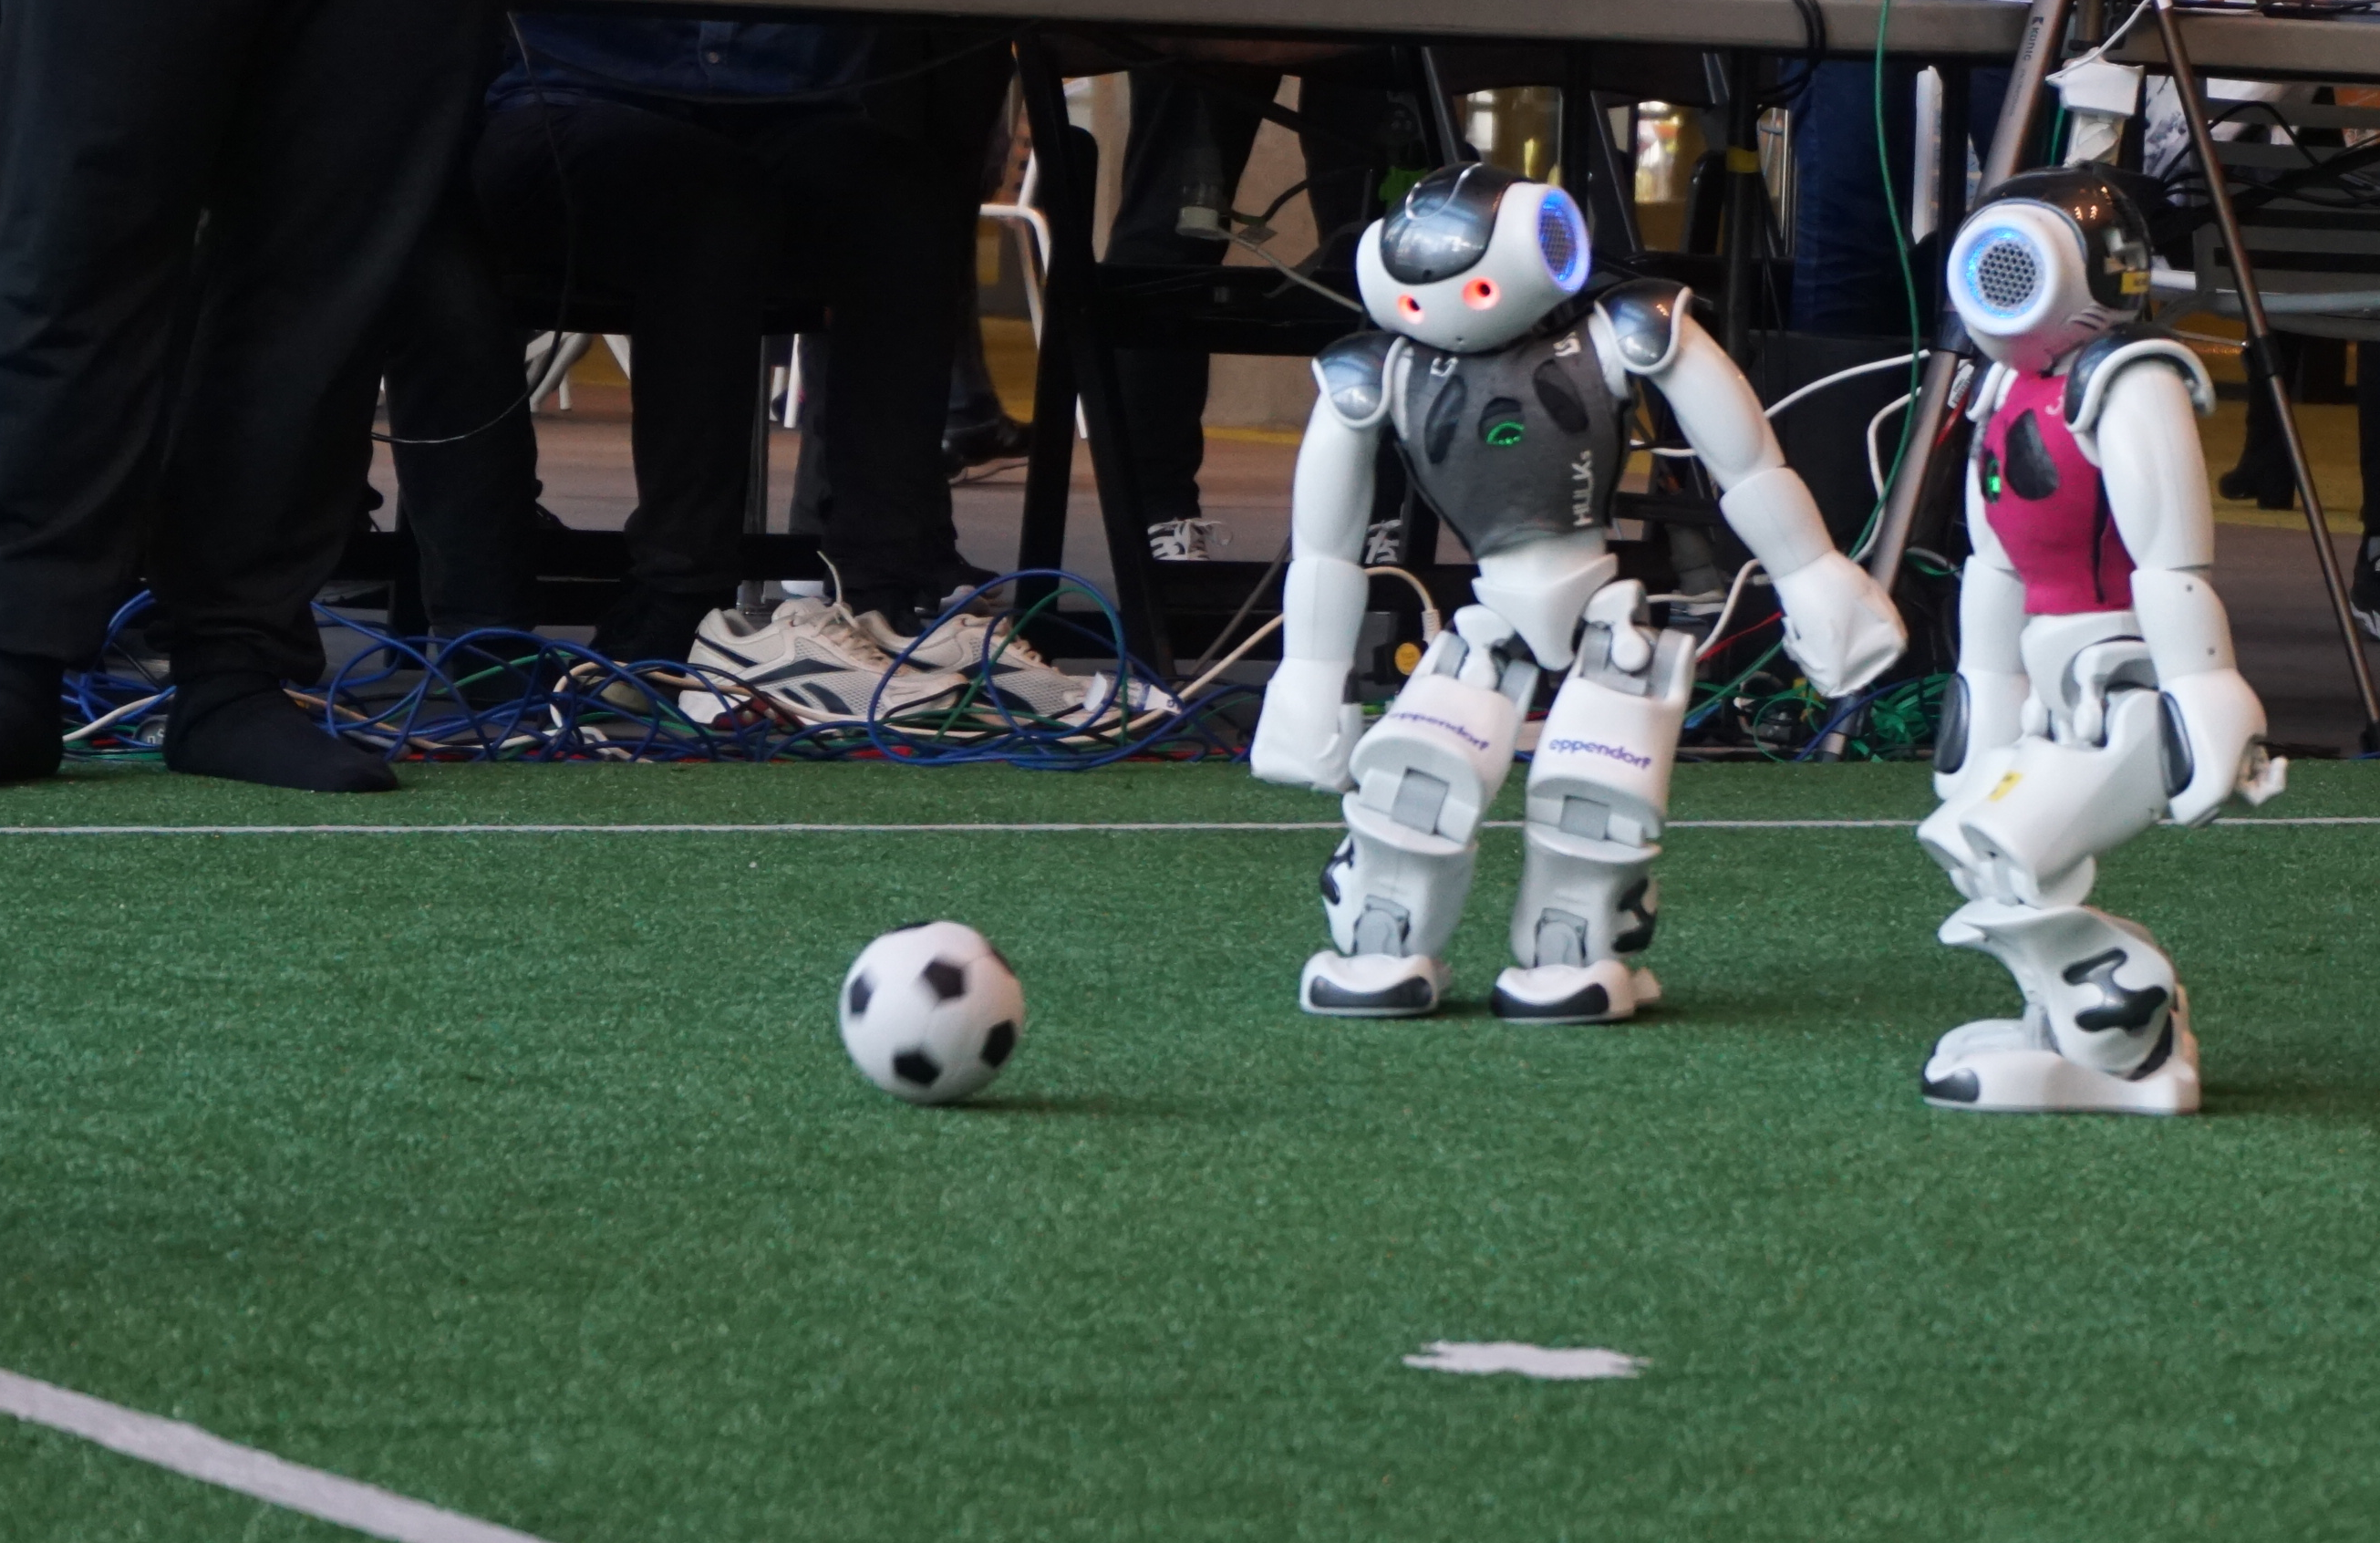
\includegraphics[width=0.6\columnwidth]{figures/robot}
	\caption[NAO robot]{V6 NAO robots while game play at the \ac{RoboCup} Sydney in 2019.}
	\label{fig:01_robot}
\end{figure}
% -------------------------------------------------------------

Within the context of the \ac{SPL}, for the \ac{RoboCup} 2019 the \textit{Directional
Whistle Challenge} was added as a technical challenge. This challenge acted as
initiator for this work. In the \ac{SPL}, technical challenges cover smaller
game independent tasks to test the realizability of concepts and to explore
preliminary ideas that might be used to inspire prospective rule changes. By
changing the rules every year, the difficulty is increased and the conditions
are adapted to reach the level of human soccer as the overarching goal until
2050. According to the current rules of the league \cite{rules},
whistles are only used for indicating the kick off of a game. However,
future considerations exist to use the whistle more frequently to mark
game state changes. Therefore, 2019's challenge required participants to
localize the position of a whistle blown by a referee with one or
multiple robots on the soccer field.
%  like executions of free kicks which include corner kicks or kick-ins.
Currently, most teams are able to reliably detect whistle sounds. However, the
issue occurs that robots detect whistles of neighboring games and therefore
start playing ahead of the own game start which yields a penalty. With
increasing importance of the whistle for the communication between the referee
and the robots, this becomes an even more pressing issue.

As another imaginable case of application, a \ac{SSL} can be used to improve team
communication among the robots.
For example, the keeper could use an audio signal to identify itself to other team
members. With an \ac{SSL} in place this signal can be localized, allowing other
team members to recognizes if they are about to score an own goal.
Potential mistakes and failure of other program components can be corrected by such
confirmation behavior between the robots.
For this reason, it was taken care of designing an algorithm that is not
limited to whistle sounds only.

\section{Contribution}
\label{sec:01_contribution}

In this work, the sixth generation of NAO robots are being used
which consists of four microphones attached on the robot's head.
For development of software for this system, an extensive framework is provided by
the \ac{SPL} team \textit{HULKs}, a group of engineering students associated
with the \ac{TUHH}.
In this software framework, a reliable detector for whistle sounds already exits.
This implementation will be utilized for the development of the \ac{SSL}. The
whistle detector of the \textit{HULKs} achieves a true positive rate of 98\si{\percent}
and has shown good performance at competitions in the past \cite{Hasselbring}, \cite{statistics}.
In practice, false positives only occur when whistles are are blown
at other fields as explained above. This emphasizes the importance of
a source localization as an useful extension to allow rejection of whistles
sounds detected from neighboring fields.
\missing[]{conditions at competition? -> large hall}

The stages required to realize the \ac{SSL} can be divided into two steps.
First, a single robot \acf{WSDE} on individual stand-alone systems estimates the
relative direction of the sound source by computing the \ac{TDOA} between
multiple microphones. After this, the single robot results are shared among the team
via wireless communication in an effort to compute the absolute sound location
from the multi-agent data.

% In the framework of the HULKs, an interface for rule compliant intra-team
% communication already exists and can be used to manage the network
% communication.\todo{All of this seems to be quite a lot of detail for a section
% titled "objective"}.

As part of this work, three \ac{TDOA} algorithms are implemented and evaluated
to identify an appropriate method to reliable estimate the relative direction
on individual robots. The standard \acf{CC} method is compared with the
\acf{GCC}, as well as a phase difference method which observes the phases of a reference
frequency between the microphones. In order to avoid reverberation and
observing multi-path propagated signals, focus is layed on the start of the
signal which is assumed to be most unaffected by these artefacts. Finally, the
objective is to provide a fully functional \ac{SSL} pipeline within the HULKs
framework that can be executed in real-time to estimate the sound location in
a global frame using a varying numbers of robots.

% say that all measurements were done in lab -> in evaluation part
% evaluation -> SSD at beginning

\section{Outline}
\label{sec:01_outline}

\Cref{chap:02_prerequisites} covers the theoretical background of this work
divided with regard to the main components of the \ac{SSL}, namely signal start detection,
\ac{WSDE} and multi-agent filtering.
In \Cref{chap:03_implementation} the implementation details are presented before
the results of the different approaches are evaluated with real data in \cref{chap:04_evaluation}.
With the outcome of this, a final conclusion is summarized in \Cref{chap:05_conclusion}.